\section{Évaluation de l'hypothèse de pertinence}
\label{section:4.4-HYPOTHESE-PERTINENCE}

	%%% Introduction / Transition.
	Jusqu'à présent, nous avons analysé la performance et l'évolution des résultats de notre implémentation du \textit{clustering} interactif à l'aide d'une vérité terrain (cf. calcul de \texttt{v-measure}).
	Cependant, une telle référence n'est pas accessible en situation réelle (l'objectif de notre méthode est précisément de la construire).
	Nous devons donc nous intéresser à d'autres moyens d'estimer la pertinence des bases d'apprentissages obtenus et de définir comment définir l'exploitabilité d'un résultat.
	Ainsi, nous aimerions vérifier l'hypothèse suivante :
	
	%%% Formulation des hypothèses:
	\begin{tcolorbox}[
		title=\faVial~\textbf{Hypothèse de pertinence}~\faVial,
		colback=colorTcolorboxHypothesis!15,
		colframe=colorTcolorboxHypothesis!75,
		width=\linewidth
	]
		« \textbf{
			Au cours d'une méthodologie d'annotation basée sur le \textit{clustering} interactif, il est possible à un expert métier d'évaluer rapidement la pertinence de la base d'apprentissage en construction sans utiliser de vérité terrain.
		} » \\
		
		% Figure.
		La figure~\ref{figure:4.4-HYPOTHESE-PERTINENCE} illustre cette hypothèse et l'espoir de pouvoir caractériser la qualité de la base d'apprentissage en cours de construction en fonction d'une valeur métier exprimée par un expert.
		%
		\begin{figure}[H]  % keep [H] to be in the tcolorbox.
			\centering
			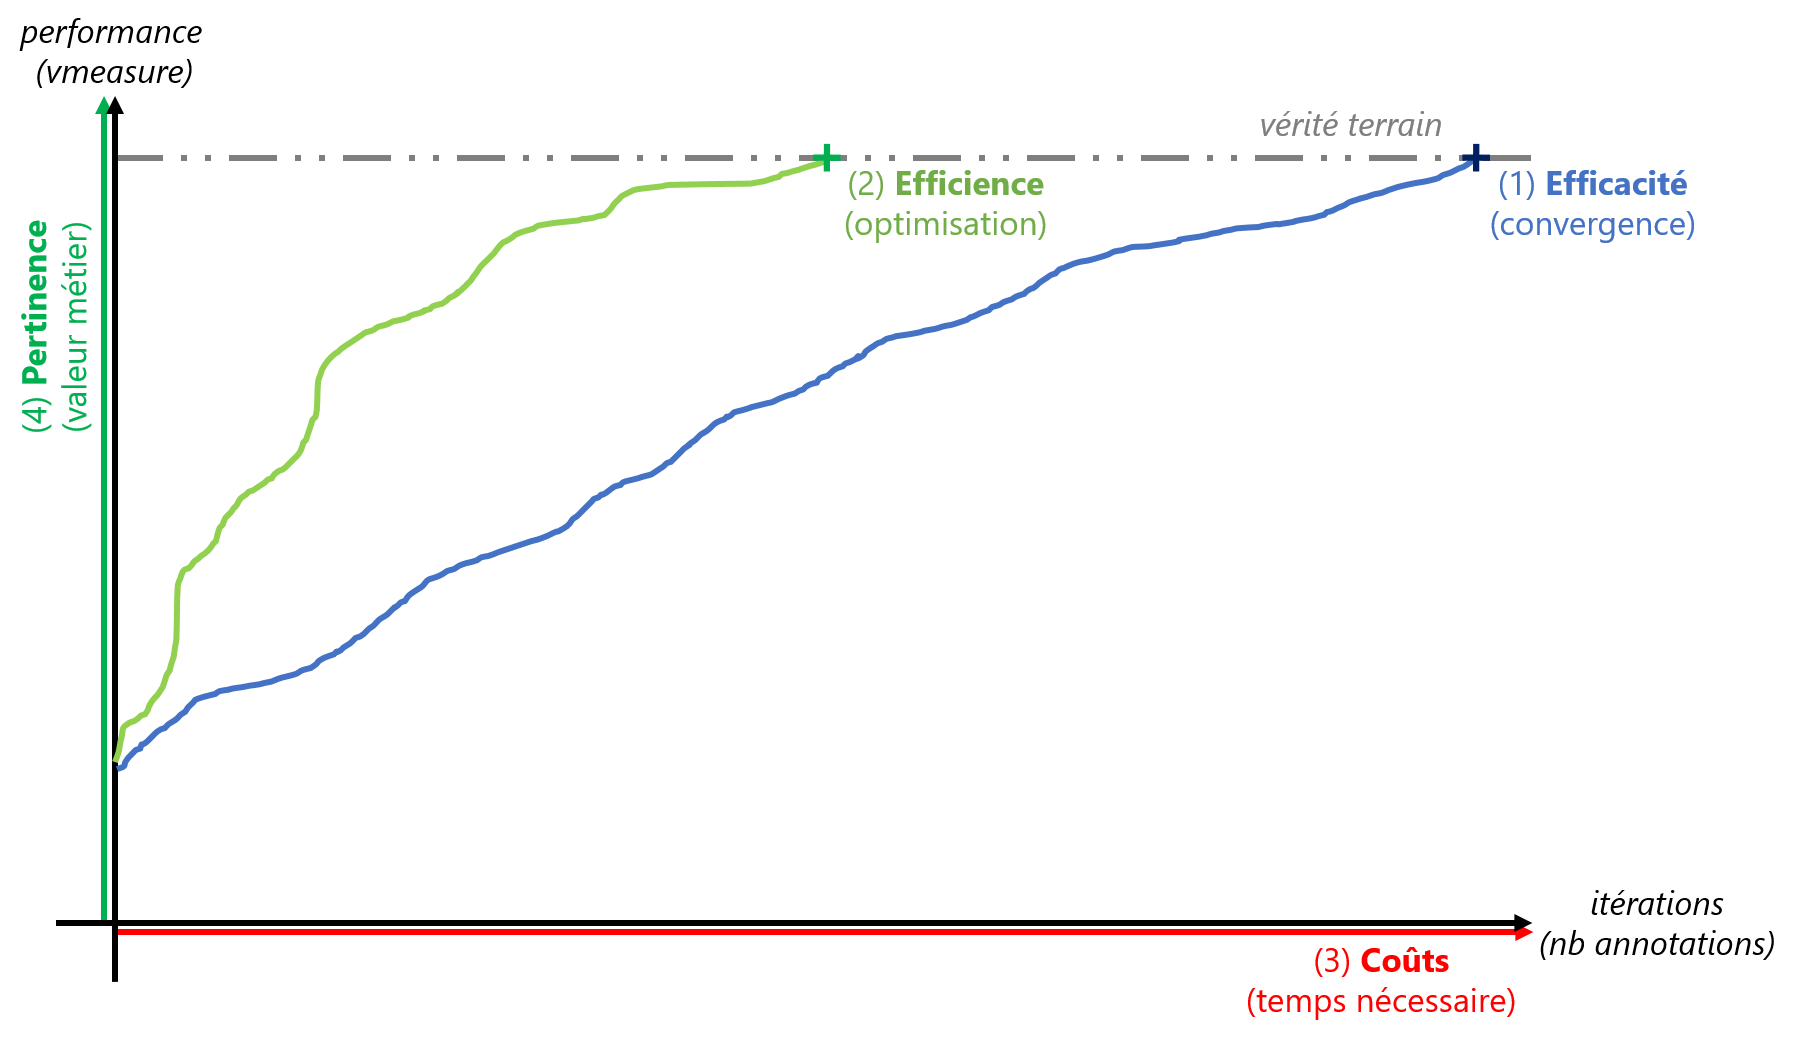
\includegraphics[width=0.95\textwidth]{figures/hypotheses-04-pertinence}
			\caption{Illustration des études réalisées sur le \textit{clustering} interactif (\textit{étape 4/6}) en schématisant l'évolution de la pertinence (\textit{valeur métier évaluée par l'expert et exprimé en nombre de clusters}) d'une base d'apprentissage en cours de construction en fonction du coût temporel de la méthode (\textit{temps nécessaire à l'expert métier et à la machine}).}
			\label{figure:4.4-HYPOTHESE-PERTINENCE}
		\end{figure}

	\end{tcolorbox}
		
	% Résumé de l'étude.
	Afin de vérifier cette hypothèse, nous explorons trois approches :
	\begin{itemize}
		\item une \textbf{vérification par un expert} du partitionnement des données obtenus, en parcourant manuellement le contenu des \textit{clusters} et en donnant un avis sur l'exploitabilité de ces derniers (cf. sous-section~\ref{section:4.4.1-ETUDE-PERTINENCE-VERIFICATION-MANUELLE}) ;
		\item une analyse des \textbf{patterns linguistiques saillants} dans la base d'apprentissage à l'aide d'une stratégie de sélection des composantes principales d'un modèle (cf. sous-section~\ref{section:4.4.2-ETUDE-PERTINENCE-PATTERNS-LINGUISTIQUES}),
		\item et une approche utilisant un \textbf{résumé automatique de thématique} par un modèle de langue, permettant de décrire succinctement le contenu des \textit{clusters} en une phrase. (cf. sous-section~\ref{section:4.4.3-ETUDE-PERTINENCE-RESUME-AUTOMATIQUE}).
	\end{itemize}
	
	
	%%%
	%%% Subsection 4.4.1: Étude d'une vérification manuelle de la valeur métier d'une base d'apprentissage par un expert
	%%%
	\subsection{Étude d'une vérification manuelle de la valeur métier d'une base d'apprentissage par un expert}
	\label{section:4.4.1-ETUDE-PERTINENCE-VERIFICATION-MANUELLE}
		
		% Objectif de l'expérience.
		Afin d'estimer la pertinence d'un résultat de \textit{clustering}, notre première intuition consiste à demander simplement l'avis d'un expert sur la base d'apprentissage en cours de construction.
		En lui posant certaines questions, nous espérons obtenir une description qualitative de chaque \textit{cluster}et ainsi déduire quand le résultat du \textit{clustering} interactif devient exploitable pour définir et entraîner un modèle de classification.
	
		%%% Protocole expérimental.
		\subsubsection{Protocole expérimental}
			
			% Pseudo-code.
			Pour résumer le protocole expérimental que nous décrivons ci-dessous, vous pouvez vous référer au pseudo-code décrit dans Alg.~\ref{algorithm:4.4.1-ETUDE-PERTINENCE-VERIFICATION-MANUELLE-PROTOCOLE}.
			%
			\begin{algorithm}[!htb]
				\begin{algorithmic}[1]
					\Require jeux de données annotés (vérité terrain) de tailles différentes
					\State \textbf{initialisation (données)}: récupérer ou générer les données et la vérité terrain
					\State \textbf{initialisation (contraintes)}: créer une liste vide de contraintes
					\State \textbf{prétraitement}: supprimer le bruit dans les données avec \texttt{prep.simple}
					\State \textbf{vectorisation}: transformer les données en vecteurs avec \texttt{vect.tfidf}
					\State \textbf{clustering initial}: regrouper les données par similarité avec \texttt{clust.kmeans.cop}
					\State \textbf{évaluation manuelle}: juger de l'exploitabilité de chaque \textit{cluster}
					\Repeat
						\State \textbf{échantillonnage}: sélectionner de nouvelles contraintes à annoter
						\State \textbf{simulation d'annotation}: ajouter des contraintes avec \texttt{samp.closest.diff}
						\State \textbf{clustering}: regrouper les données par similarité avec \texttt{clust.kmeans.cop}
						\State \textbf{évaluation manuelle}: juger de l'exploitabilité de chaque \textit{cluster}
						\State \textbf{labellisation manuelle}: nommer chaque \textit{cluster} exploitable
					\Until{annotation de toutes les contraintes possibles}
					\State \textbf{analyse}: afficher l'évolution de l'exploitabilité de chaque itération de \textit{clustering}
					\Ensure discussion sur la complexité de la tâche et sur l'évolution de l'exploitabilité
				\end{algorithmic}
				\caption{Description en pseudo-code du protocole expérimental de l'étude de vérification manuelle de la valeur métier d'une base d'apprentissage.}
				\label{algorithm:4.4.1-ETUDE-PERTINENCE-VERIFICATION-MANUELLE-PROTOCOLE}
			\end{algorithm}
			
			% Description de la vérité terrain.
			Nous utilisons comme vérité terrain le jeu de données \texttt{Bank Cards (v1.0.0)} : ce dernier traite des demandes les plus fréquentes des clients en ce qui concerne la gestion de leur carte bancaire.
			Il est composé de $500$ questions rédigées en français et réparties en $10$ classes (\texttt{perte ou vol de carte}, \texttt{carte avalée}, \texttt{commande de carte}, ...).
			Pour plus de détails, consultez l'annexe~\ref{annex:C.1-DATASET-BANK-CARDS}.
			
			% Description des tentatives de la méthode.
			Sur ce jeu de données, nous exécutons une tentative complète
			\footnote{Tentative complète : itérations d'échantillonnage, d'annotation et de \textit{clustering} jusqu'à annotation de toutes les contraintes possibles.}
			de la méthode du \textit{clustering} interactif utilisant notre paramétrage favori, et cette tentative est répétée $5$ fois pour contrer les aléas statistiques des exécutions.
			
			% Description de l'évaluation manuelle.
			Au cours des itérations, un expert qualifie chaque \textit{cluster} en donnant son avis sur sa valeur métier.
			Afin d'encadrer ses réponses, nous lui demandons d'analyser trois aspects :
			\begin{itemize}
				\item est-ce que le \textit{cluster} a une thématique principale \textbf{bien définie} ? (\textit{en effet, comment interpréter un cluster sans définition claire ?})
				\item est-ce que le \textit{cluster} est constitué par un nombre suffisant de données ? (\textit{en effet, comment entraîner un modèle de classification sans données ?})
				\item est-ce que le \textit{cluster} n'est pas trop bruité ? (\textit{en effet, comment avoir de bonnes performances si la base d'apprentissage n'est pas fiable ?})
			\end{itemize}
			
			L'avis exprimé par l'expert métier est alors classé en trois niveaux :
			\begin{itemize}
				\item \textbf{exploitable} : le \textit{cluster} possède (1) une thématique bien définie, (2) un nombre de données suffisant pour entraîner un modèle de classification et (3) peu de bruit ; ce \textit{cluster} peut donc être exploité en l'état ou avec peu de modifications manuelles ;
				\item \textbf{partiellement exploitable} : soit le \textit{cluster} est composé de plusieurs de thématiques (\textit{deux ou trois}), soit il ne comporte pas pas assez de données (\textit{moins d'une vingtaines}), soit il est bruité (\textit{au moins un quart de bruit}) ; ce \textit{cluster} donne une première base pour créer une classe, mais un travail manuel est nécessaire (\textit{ajout de données, tri du bruit, ...}) ;
				\item \textbf{non exploitable} : soit le \textit{cluster} ne contient pas ou contient trop de thématique, soit c'est un \textit{cluster} singleton ou un \textit{cluster} poubelle, soit ce \textit{cluster} est complètement bruité ; dans tous les cas, il n'est absolument pas exploitable sans un gros travail manuel.
			\end{itemize}
			
			Pour limiter la charge de travail de l'opérateur, nous ne demandons l'expertise que toutes les $5$ itérations d'une tentative.
			
			% Référence scripts.
			\begin{leftBarInformation}
				Les scripts de l'expérience, réalisés avec des \textit{notebooks} Python (\cite{van-rossum-drake:2009:python-reference-manual}), sont disponibles dans un dossier dédié de~\cite{schild:2021:cognitivefactory-interactiveclusteringcomparativestudy}.
			\end{leftBarInformation}
			

		%%% Résultats
		\subsubsection{Résultats obtenus}
			
			% Axiome/Contraintes.
			\begin{leftBarWarning}
				Par manque de personnes aptes à qualifier le jeu de données utilisé, les annotations réalisées dans cette étude n'ont pu être faites que par un seul annotateur.
				Malgré cette contrainte, nous supposons que la réalisation de l'analyse sur $5$ tentatives différentes de la méthode permet de limiter les biais et de discuter des tendances générales.
			\end{leftBarWarning}
		
			% Description statistiques.
			La figure~\ref{figure:4.4.1-ETUDE-PERTINENCE-VERIFICATION-MANUELLE} met en avant l'évolution de le pertinence moyenne estimée par l'opérateur sur la base des contenu des \textit{clusters}.
			Nous allons nous intéresser à trois phases s'y distinguant.
			
			% 0: Initialisation
			À l'initialisation (itération $0$), la majeure partie des \textit{clusters} sont inexploitables (environ $60$\%) et seul $35$\% d'entre eux semblent exploitables.
			Dans le top $3$ des classes facilement identifiables à ce stade, nous retrouvons \texttt{gestion\_sans\_contact} ($5/5$), \texttt{consultation\_solde} ($3/5$) et \texttt{gestion\_carte\_virtuelle} ($3/5$).
			
			% 0-10: Phase d'exploration.
			Nous constatons ensuite une première phase de remaniement des \textit{clusters}, située entre les itérations $0$ et $10$, où le taux d'inexploitables chute au profit des \textit{clusters} partiellement exploitables, dont la proportion augmente de $10$ à près de $40$\%.
			À l'itération $10$, le top $3$ des classes identifiables mais bruitées ou en cohabitation dans un \textit{cluster} sont \texttt{gestion\_carte\_virtuelle} ($4/5$),  \texttt{alerte\_perte\_vol\_carte} ($4/5$) et  \texttt{commande\_carte} ($4/5$).
			
			% 10-25: Phase de consolidation.
			Une seconde phase de consolidation se présente entre les itérations $10$ et $25$.
			Durant cette phase, les taux de \textit{clusters} non exploitables et de partiellement exploitables diminuent alors que le taux d'exploitables monte en flèche (de $35$\% à $90$\% en $15$ itérations).
			La majeure partie des \texttt{clusters} sont ainsi exploitables en l'état ou après la correction de quelques points aberrants.
			Après l'itération $25$, le \textit{cluster} le plus récalcitrant concerne un mélange des classes \texttt{alerte\_perte\_vol\_carte} et \texttt{gestion\_decouvert} ($5/5$).

			% Figure.
			\begin{figure}[!htb]
				\centering
				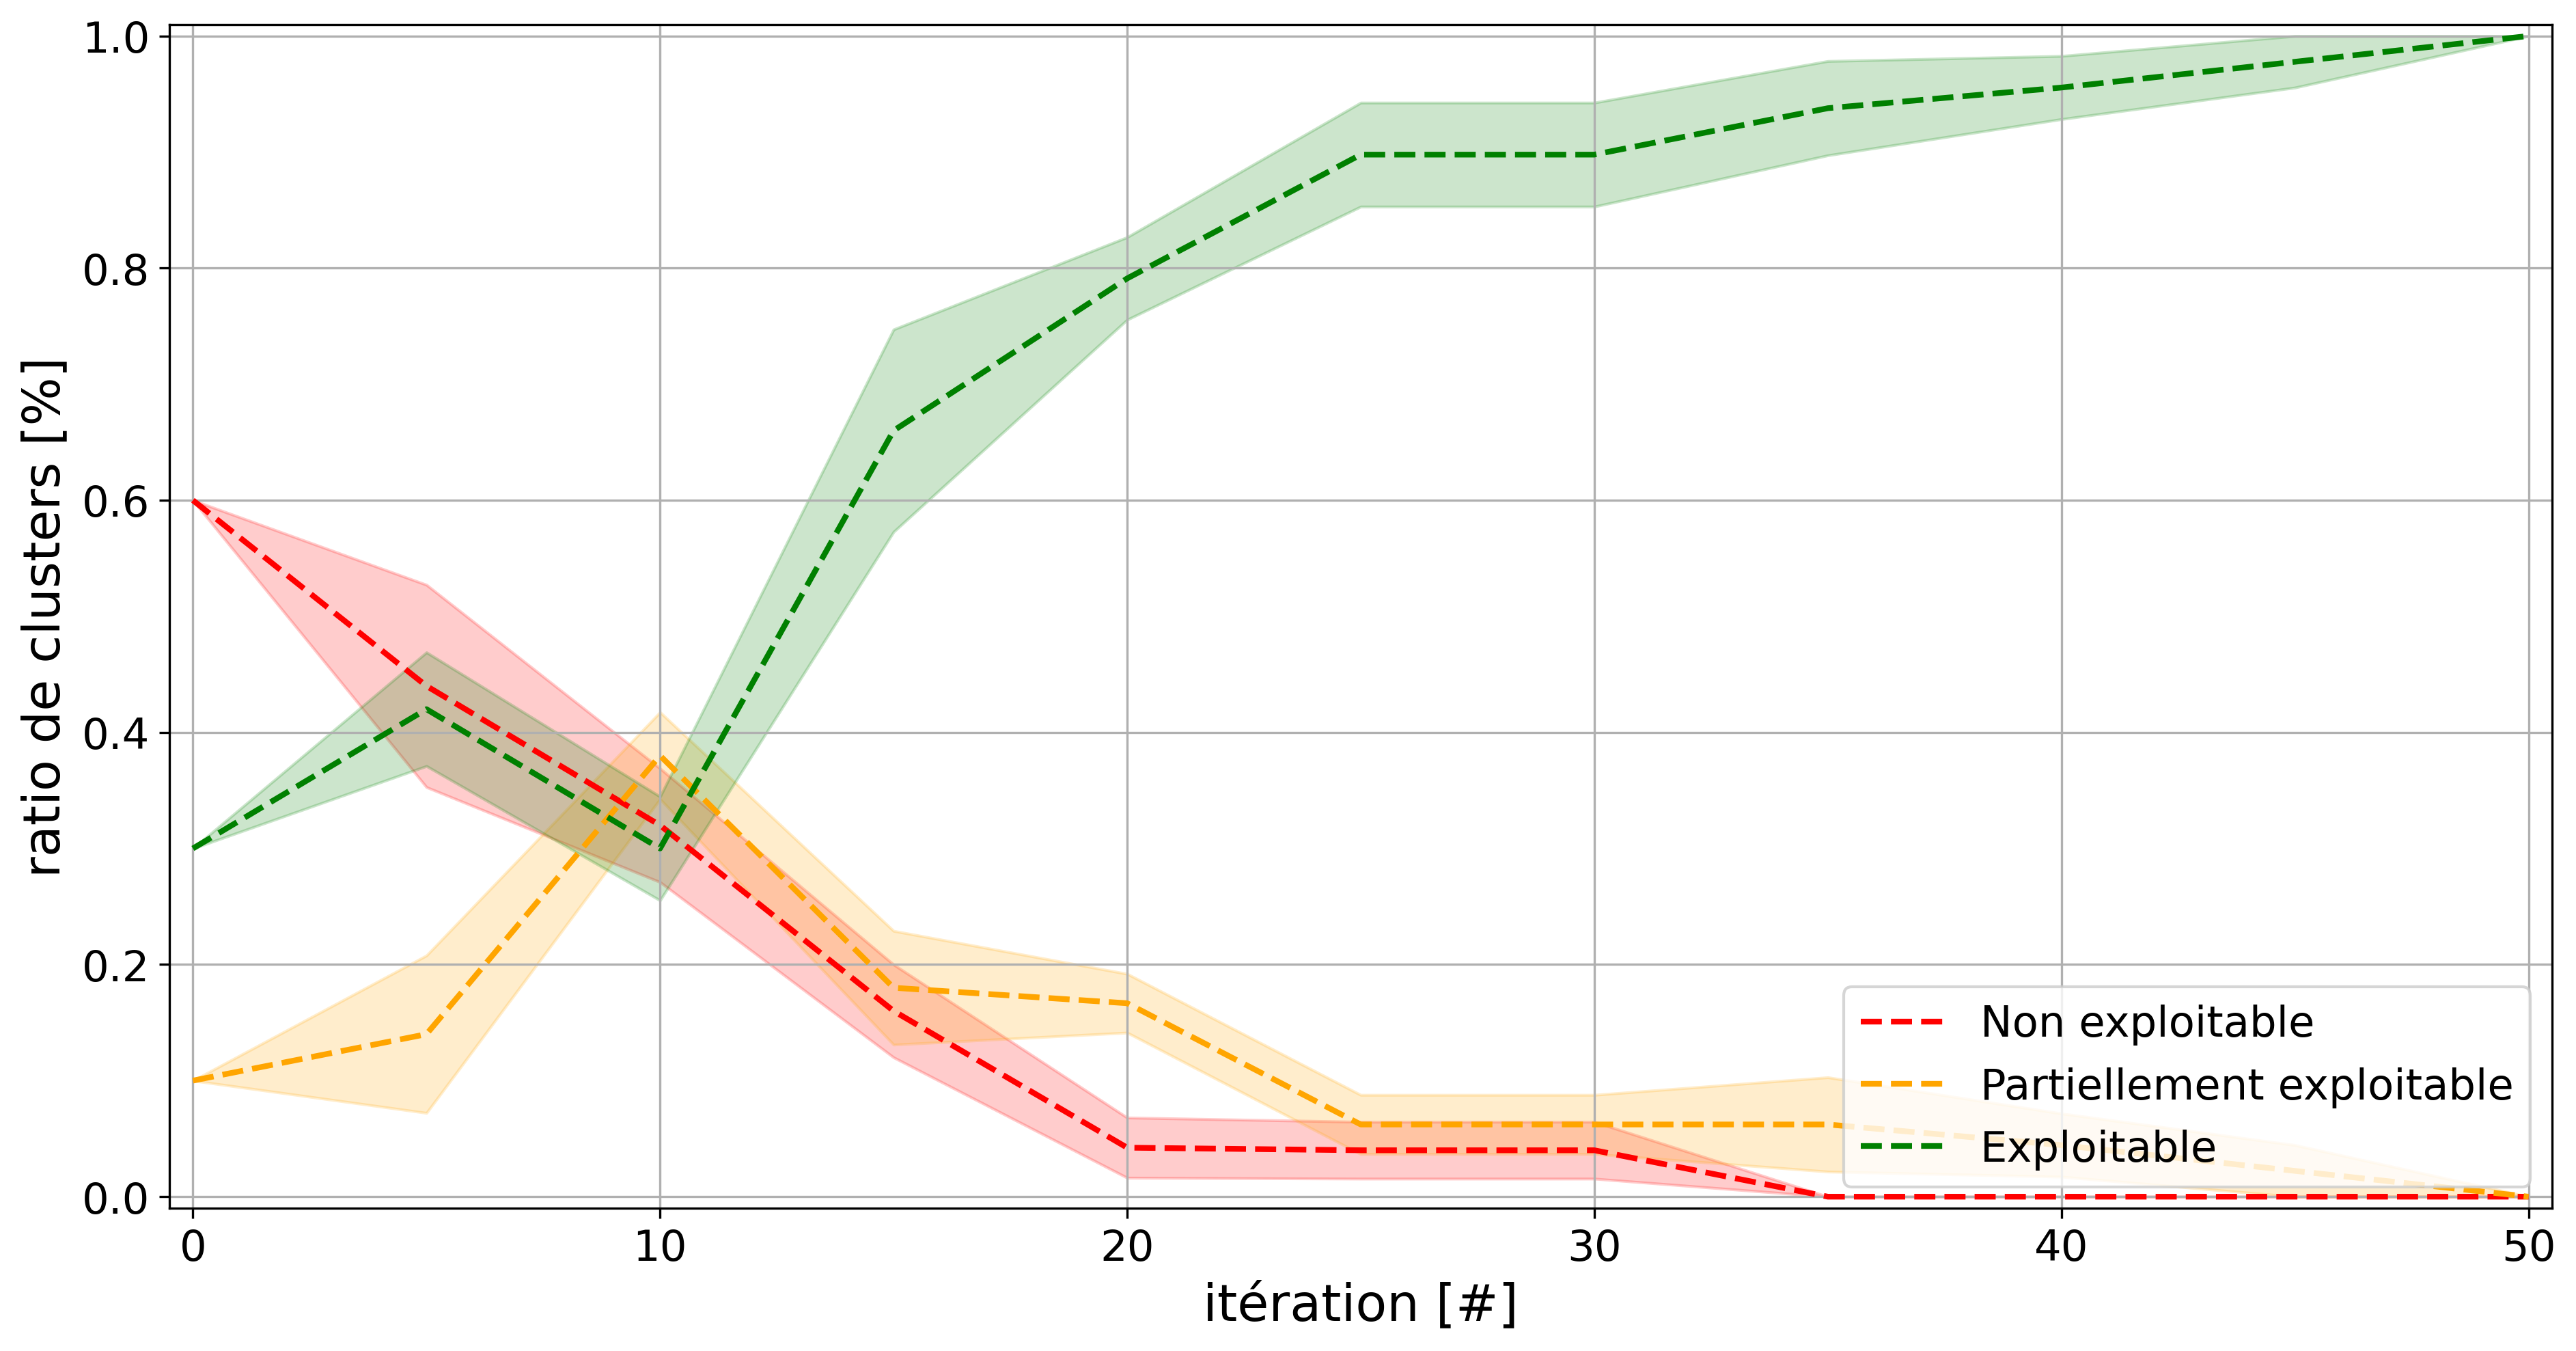
\includegraphics[width=0.95\textwidth]{figures/etude-pertinence-llm-check-clustering-annotation-favori}
				\caption{Évolution de la pertinence métier moyenne estimée manuellement au cours des itérations du résultat du \textit{clustering} interactif avec notre paramétrage favori.
				Cette pertinence, exprimée en proportion du nombre de \textit{clusters}, est retranscrite en trois niveaux : \texttt{exploitable} en vert, \texttt{partiellement exploitable} en orange, et \texttt{non exploitable} en rouge.}
				\label{figure:4.4.1-ETUDE-PERTINENCE-VERIFICATION-MANUELLE}
			\end{figure}


		%%% Discussion
		\subsubsection{Discussion}
		
			% Rappel de l'objectif.
			Cette première étude visait à observer comment un expert métier peut interpréter un résultat de \textit{clustering} proposé par notre méthode.
			
			% Remarques sur l'évolution de l'exploitabilité.
			Comme l'analyse n'a pu être faite que par un seul opérateur, nous ne nous attarderons pas sur la précision des taux d'exploitabilité des clusters.
			Nous pouvons déjà reconnaître que trois phases sont présentes :
			\begin{itemize}
				\item une première \textbf{phase exploratoire} (cf. itérations $0$ à $10$), où de premiers \textit{clusters} partiellement exploitables apparaissant.
				Ces derniers contiennent souvent une thématique bruitée ou quelques thématiques mal séparées, ce qui permet toutefois à l'expert de se faire une idée des thématiques contenu dans la collecte de données.
				Cependant, s'arrêter à ce stade demanderait beaucoup de travail manuel pour obtenir une base d'apprentissage opérationnelle ;
				\item une seconde \textbf{phase de consolidation} (cf. itérations $10$ à $25$), où les \textit{clusters} partiellement exploitable se raffinent.
				De plus en plus de \textit{clusters} bien définis naissent, avec une seul thématique et peu de bruits.
				Ces derniers pourraient être extraits et exploités en l'état ;
				\item une \textbf{phase de parachèvement} (cf. itérations après $25$), où la plupart des \textit{clusters} sont exploitables en l'état mais quelques-uns nécessitent encore du travail.
				Cette phase est la moins rentable car les derniers \textit{clusters} et points aberrants sont corrigés petit à petit, mais sans impact notable sur leur valeur métier. 
			\end{itemize}
			
			% Remaques expérience utilisateur : tâche complexe.
			Au cours de ces vérifications, il apparaît que la complexité réside dans l'analyse des \textit{clusters} partiellement exploitables.
			En effet, les clusters totalement exploitable ou totalement inexploitables sont souvent simples à identifier.
			les premiers se repèrent facilement, surtout quand ils sont déjà présents lors d'itérations précédentes (exemple de la classe \texttt{gestion\_sans\_contact}, présente dès l'itération $0$) ;
			les seconds, plutôt présents au début de la méthode, peuvent mélanger un grand nombre de thématique et s'apparenter rapidement à des \textit{clusters} poubelle.
			En revanche, les \textit{clusters} partiellement exploitables peuvent avoir des limites subjectives, alterant parfois l'avis de l'expert.
			
			% Remaques expérience utilisateur : tâche complexe.
			Pour aller plus loin, la difficulté de cette tâche est aussi dû aux contraintes suivantes :
			\begin{itemize}
				\item il faut être capable de maintenir en mémoire de grands ensembles de données ;
				\item il faut estimer la thématique principale à l'aide de données désordonnées ;
				\item il faut examiner la cohérence de cette thématique alors que le vocabulaire employé diffère ;
				\item il faut juger de l'importance du bruit contenu dans les \textit{clusters} ;
				\item il faut prendre du recul pour repérer la dispersion d'une thématique dans plusieurs \textit{clusters} ;
				\item ...
			\end{itemize}
			Tous ces facteurs peuvent donc nuire à la qualité, tant sur l'estimation de l'exploitabilité que sur le nommage des \textit{clusters}.
			
			% Remarques expérience utilisateur : impacts sur la qualité.
			Ainsi, nous déduisons aisément que l'expérience utilisateur proposée à l'expert métier n'est pas séduisante.
			Comme l'analyse de l'exploitabilité d'un \textit{cluster} semble être une tâche complexe, il semble inconcevable de demander sa réalisation sur tous les \textit{clusters} de toutes les itérations !
			De plus, sans aide supplémentaire et sans vis-à-vis pour se confronter à ses conclusions d'analyse, l'opérateur peut difficilement vérifier la cohérence et la reproductibilité de son travail.
			Il est donc nécessaire de considérer des pistes d'amélioration pour ne pas abandonner l'expert métier à lui-même dans cette tâche cruciale.
			
			% Conclusions et suggestion.
			Quelques pistes peuvent être étudier pour accompagner l'opérateur :
			\begin{itemize}
				\item employer plusieurs experts pour valider par consensus leurs appréciation sur un résultat de \textit{clustering} : cette méthode est efficace pour rattraper les thématiques non identifiées et pour s'accorder sur la valeur d'un \textit{cluster} ;
				\item prémâcher le travail d'analyse en réalisant une étude linguistique des \textit{clusters}, et permettre ainsi d'identifier grossièrement les thématiques présentes en fonction du vocabulaire employé (cf. sous-section~\ref{section:4.4.2-ETUDE-PERTINENCE-PATTERNS-LINGUISTIQUES}) ;
				\item automatiser une partie du travail d'analyse en utilisant les capacités des larges modèles de langue, afin d'alléger la charge de travail demandée aux experts métiers (cf. sous-section~\ref{section:4.4.3-ETUDE-PERTINENCE-RESUME-AUTOMATIQUE}).
			\end{itemize}
	
	
	%%%
	%%% Subsection 4.4.2: Etude des patterns linguistiques pertinents à l'aide de la \textit{Features Maximization}
	%%%
	\subsection{Étude des patterns linguistiques pertinents à l'aide de la \textit{Features Maximization}}
	\label{section:4.4.2-ETUDE-PERTINENCE-PATTERNS-LINGUISTIQUES}
		
		% Objectif de l'expérience.
		Nous venons de conclure que la vérification manuelle d'un résultat de \textit{clustering} interactif est fonctionnelle, mais qu'elle souffre d'une très mauvaise expérience utilisateur.
		Afin d'améliorer cette aspect, une première idée consiste à mettre en valeur le vocabulaire caractéristique de chaque \textit{cluster} et d'examiner si ces informations sont utiles à l'appréciation de leur valeur métier.
	
		%%% Protocole expérimental.
		\subsubsection{Protocole expérimental}
			
			% Pseudo-code.
			Pour résumer le protocole expérimental adapté, vous pouvez vous référer au pseudo-code décrit dans Alg.~\ref{algorithm:4.4.2-ETUDE-PERTINENCE-PATTERNS-LINGUISTIQUES-PROTOCOLE}.
			%
			\begin{algorithm}[!htb]
				\begin{algorithmic}[1]
					\Require jeux de données annotés (vérité terrain) de tailles différentes
					\State \textbf{initialisation (données)}: récupérer ou générer les données et la vérité terrain
					\State \textbf{initialisation (contraintes)}: créer une liste vide de contraintes
					\State \textbf{prétraitement}: supprimer le bruit dans les données avec \texttt{prep.simple}
					\State \textbf{vectorisation}: transformer les données en vecteurs avec \texttt{vect.tfidf}
					\State \textbf{clustering initial}: regrouper les données par similarité avec \texttt{clust.kmeans.cop}
					\State \textbf{évaluation manuelle}: juger de l'exploitabilité de chaque \textit{cluster}
					\Repeat
						\State \textbf{échantillonnage}: sélectionner de nouvelles contraintes à annoter
						\State \textbf{simulation d'annotation}: ajouter des contraintes avec \texttt{samp.closest.diff}
						\State \textbf{clustering}: regrouper les données par similarité avec \texttt{clust.kmeans.cop}
						\State \textbf{analyse linguistique}: déterminer le vocabulaire caractéristique de chaque cluster
						\State \textbf{évaluation semi-manuelle}: juger de l'exploitabilité de chaque \textit{cluster}
						\State \textbf{labellisation manuelle}: nommer chaque \textit{cluster} exploitable
					\Until{annotation de toutes les contraintes possibles}
					\State \textbf{analyse}: afficher l'évolution de l'exploitabilité de chaque itération de \textit{clustering}
					\Ensure discussion sur la complexité de la tâche et sur l'évolution de l'exploitabilité
				\end{algorithmic}
				\caption{Description en pseudo-code du protocole expérimental de l'étude des patterns linguistiques pertinents pour vérifier la valeur métier d'une base d'apprentissage.}
				\label{algorithm:4.4.2-ETUDE-PERTINENCE-PATTERNS-LINGUISTIQUES-PROTOCOLE}
			\end{algorithm}
			
			% Détails de l'expérience.
			Nous nous appuyons sur le même protocole que l'expérience précédente (sous-section~\ref{section:4.4.1-ETUDE-PERTINENCE-VERIFICATION-MANUELLE}) : nous utilisons donc comme vérité terrain le jeu de données \texttt{Bank Cards (v1.0.0)}, nous réalisons $5$ tentatives complètes de la méthode du \textit{clustering} interactif utilisant notre paramétrage favori, et nous demandons toutes les $5$ itérations à un expert de qualifier les \textit{clusters} obtenus entre trois catégories (\textbf{exploitable}, \textbf{partiellement exploitable} et \textbf{non exploitable}).
			
			% Ajout de l'analyse linguistique.
			Cependant, avant de demander l'avis de l'expert, nous réalisons une analyse du vocabulaire employé.
			Pour cela, nous utilisons une sélection des patterns linguistiques pertinents basée sur la maximisation des traits (notée \texttt{FMC}, cf.~\cite{lamirel-etal:2017:novel-approach-feature}) : cette méthode permet de trouver des composantes caractéristiques et discriminantes de chaque \textit{cluster} en attribuant un score à chaque couple $(\texttt{cluster}, \texttt{mot})$.
			À l'aide de cette analyse statistique, nous pouvons ainsi mettre en avant des mots clés du \textit{cluster} et surligner ces mots dans les questions à parcourir.
			
			% Description de l'évaluation semi-manuelle.
			Nous adaptons aussi la tâche de l'expert afin qu'il donne son avis sur chaque \textit{cluster} en répondant aux questions suivantes :
			\begin{itemize}
				\item est-ce que la liste des patterns linguistiques caractéristiques du \textit{cluster} est suffisamment complète pour permettre d'identifier une thématique principale \textbf{bien définie} ? (\textit{en effet, comment interpréter un cluster sans définition claire ?})
				\item est-ce que la liste des patterns linguistiques caractéristiques du \textit{cluster} identifie plusieurs thématiques ou bruits dans le \textit{cluster} ? (\textit{en effet, comment avoir de bonnes performances si la base d'apprentissage n'est pas fiable ?})
			\end{itemize}
			
			\begin{leftBarIdea}
				Nous pourrions aussi analyser l'impact ergonomique qu'apporte la mise en exergue des patterns linguistiques pertinents dans le texte de chaque \textit{cluster}.
				Cette étude pourrait ainsi mesurer le gain de temps et de qualité par rapport à une vérification manuelle non assistée comme présentée en sous-section~\ref{section:4.4.1-ETUDE-PERTINENCE-VERIFICATION-MANUELLE}.
			\end{leftBarIdea}
			
			% Référence scripts.
			\begin{leftBarInformation}
				Les scripts de l'expérience, réalisés avec des \textit{notebooks} Python (\cite{van-rossum-drake:2009:python-reference-manual}), sont disponibles dans un dossier dédié de~\cite{schild:2021:cognitivefactory-interactiveclusteringcomparativestudy}.
				L'implémentation de la maximisation des traits est accessible ici dans~\cite{schild:2023:cognitivefactory-featuresmaximizationmetric}.
			\end{leftBarInformation}

		%%% Résultats
		\subsubsection{Résultats obtenus}
			
			% Axiome/Contraintes.
			\begin{leftBarWarning}
				Par manque de moyen, la relecture manuelle des \textit{clusters} n'a pas été réalisée.
				Nous présentons donc simplement quelques exemples d'analyses linguistiques réalisées grâce à la FMC.
			\end{leftBarWarning}
			
			% Description de deux cas d'études.
			Prenons quelques \textit{clusters} et suivons l'évolution de leur analyse linguistiques au cours des itérations.
			Nous nous référons aux tableaux ci-contre pour afin le top $10$ des termes caractéristiques des \textit{clusters} ainsi qu'un extrait de questions issus de ces \textit{clusters} avec une mise en évidence des termes caractéristiques dans le texte.
			
			% Exemple d'un cluster qui est bien formé dès le début.
			D'abord, prenons l'exemple suivi dans le tableau~\ref{table:4.4.2-ETUDE-PERTINENCE-PATTERNS-LINGUISTIQUES-GESTION-SANS-CONTACT}.
			Nous suivons ici l'évolution d'un \textit{cluster} bien formé dès l'itération $0$.
			En effet, il aisé de juger ce \textit{cluster} exploitable et d'en déduire sa thématique : le \textit{cluster} est de taille suffisante (plus de $45$ questions), son vocabulaire caractéristique est fourni ($36$ à $38$ patterns) et la liste des patterns mis en avant sont cohérents (\textit{sans contact}, \textit{paiement sans contact}, \texttt{activer le}, \textit{nfc}, ...).
			En parcourant son contenu, on arrive rapidement à associer sa thématique à la classe \texttt{gestion\_sans\_contact} de la vérité terrain.
			
			\begin{table}[!htb]
				\begin{center}
				\def\arraystretch{0.8}
				\begin{tabular}{|c|l|l|}
					\hline
					% ENTETE DU TABLEAU
					\multicolumn{1}{|c|}{\shortstack[c]{
						Identification \\ du cluster
					}}
						& \multicolumn{1}{c|}{\shortstack[c]{
							Analyse \\ linguistique (FMC)
						}}
						& \multicolumn{1}{c|}{\shortstack[c]{
							Aperçu du cluster \\ (avec emphase)
						}}
						\tabularnewline
						\hline
					
					% Exemple 1:
					\multirow{10}{*}{\shortstack[c]{
						{ \footnotesize Tentative: $1$ } \\
						{ \footnotesize Itération: $0$ } \\
						{ \footnotesize Cluster: $0$ } \\
						\_\_\_\_\_ \\
						{ \footnotesize Avis initial: } \\
						{ \footnotesize \color{colorDarkPastelGreen} \texttt{Exploitable} }
					}}
						& { \scriptsize - sans contact }
						& { \scriptsize - \textbf{activer le} moyen de \textbf{paiement nfc} \textbf{sur ma carte} gold }
						\tabularnewline
						
						& { \scriptsize - contact }
						& { \scriptsize - \textbf{enlever} le \textbf{mode} \textbf{sans contact} de ma carte }
						\tabularnewline
						
						& { \scriptsize - sans }
						& { \scriptsize - gerer le \textbf{mode} de \textbf{paiement nfc} \textbf{sur ma carte} }
						\tabularnewline
						
						& { \scriptsize - mode }
						& { \scriptsize - je souhaite gerer le \textbf{mode} nfc sur mes cartes bancaires }
						\tabularnewline
						
						& { \scriptsize - le mode }
						& { \scriptsize - l option \textbf{sans contact} \textbf{ne fonctionne pas} \textbf{sur ma carte} }
						\tabularnewline
						
						& { \scriptsize - sur ma carte }
						& { \scriptsize - modifier le \textbf{mode} \textbf{sans contact} }
						\tabularnewline
						
						& { \scriptsize - le sans contact }
						& { \scriptsize - modifier le \textbf{mode} nfc \textbf{sur ma carte} de paiement }
						\tabularnewline
						
						& { \scriptsize - le sans }
						& { \scriptsize - peut on annuler le paiement \textbf{sans contact} }
						\tabularnewline
						
						& { \scriptsize - paiement sans contact }
						& { \scriptsize - puis je \textbf{activer le} \textbf{sans contact} depuis l application }
						\tabularnewline
						
						& \multicolumn{1}{c|}{
							\scriptsize (Total: 36)
						}
						& \multicolumn{1}{c|}{
							\scriptsize (Total: 46)
						}
						\tabularnewline
						\hline
					
					% Exemple 2:
					\multirow{10}{*}{\shortstack[c]{
						{ \footnotesize Tentative: $1$ } \\
						{ \footnotesize Itération: $15$ } \\
						{ \footnotesize Cluster: $0$ } \\
						\_\_\_\_\_ \\
						{ \footnotesize Avis initial: } \\
						{ \footnotesize \color{colorDarkPastelGreen} \texttt{Exploitable} }
					}}
						& { \scriptsize - sans contact }
						& { \scriptsize - \textbf{activer le} moyen de paiement \textbf{nfc} \textbf{sur ma} carte gold }
						\tabularnewline
						
						& { \scriptsize - contact }
						& { \scriptsize - \textbf{enlever} le \textbf{mode} \textbf{sans contact} de ma carte }
						\tabularnewline
						
						& { \scriptsize - sans }
						& { \scriptsize - gerer le \textbf{mode} de paiement \textbf{nfc} \textbf{sur ma} carte }
						\tabularnewline
						
						& { \scriptsize - sur ma }
						& { \scriptsize - je souhaite gerer le \textbf{mode} \textbf{nfc} sur mes cartes bancaires }
						\tabularnewline
						
						& { \scriptsize - mode }
						& { \scriptsize - l \textbf{option} \textbf{sans contact} ne fonctionne pas \textbf{sur ma} carte }
						\tabularnewline
						
						& { \scriptsize - le mode }
						& { \scriptsize - modifier le \textbf{mode} \textbf{sans contact} }
						\tabularnewline
						
						& { \scriptsize - sur ma carte }
						& { \scriptsize - modifier le \textbf{mode} \textbf{nfc} \textbf{sur ma carte de paiement} }
						\tabularnewline
						
						& { \scriptsize - nfc }
						& { \scriptsize - peut on annuler le paiement \textbf{sans contact} }
						\tabularnewline
						
						& { \scriptsize - le sans contact }
						& { \scriptsize - puis je \textbf{activer le} \textbf{sans contact} depuis l application }
						\tabularnewline
						
						& \multicolumn{1}{c|}{
							\scriptsize (Total: 38)
						}
						& \multicolumn{1}{c|}{
							\scriptsize (Total: 50)
						}
						\tabularnewline
						\hline
					
				\end{tabular}
				\end{center}
				\caption{extrait de l'évolution de l'analyse linguistique du \textit{cluster} ...}
				\label{table:4.4.2-ETUDE-PERTINENCE-PATTERNS-LINGUISTIQUES-GESTION-SANS-CONTACT}
			\end{table}
			
			% Exemple d'un cluster qui se forme.
			Ensuite, prenons l'exemple décrit dans le tableau~\ref{table:4.4.2-ETUDE-PERTINENCE-PATTERNS-LINGUISTIQUES-DEBLOCAGE-CARTE}.
			A l'itération $0$, il est impossible d'exploiter ce \textit{cluster} : il n'y a que deux patterns mis en avant ne traitant pas d'une ma thématique, et les questions semblent toutes traiter de sujets différents.
			A l'itération $10$, le résultat semble un peu plus exploitable.
			Nous pouvons d'ailleurs déduire deux thématiques principales : la première, mise en avant par des patterns linguistiques de type "\textit{numero}", "\textit{online}",  et "\textit{de carte virtuelle}", permet d'imaginer un sujet sur la gestion des numéro de cartes virtuelles ; la seconde, identifiée par les termes "\textit{débloquer}" et "\textit{réactiver}", oriente plutôt vers la création d'un thème pour débloquer une carte bancaire.
			Quelques bruits sont présent, mais ce \textit{cluster} à l'itération $10$ peut donc être associé aux classes \texttt{gestion\_carte\_virtuelle} et \texttt{deblocage\_carte}.
			Dès l'itération $15$, ces thématiques se séparent en deux clusters ($2$ et $3$) : nous pouvons les identifier à l'aide de leurs listes de termes bien fournies.
			
			\begin{table}[!htb]
				\begin{center}
				\def\arraystretch{0.8}
				\begin{tabular}{|c|l|l|}
					\hline
					% ENTETE DU TABLEAU
					\multicolumn{1}{|c|}{\shortstack[c]{
						Identification \\ du cluster
					}}
						& \multicolumn{1}{c|}{\shortstack[c]{
							Analyse \\ linguistique (FMC)
						}}
						& \multicolumn{1}{c|}{\shortstack[c]{
							Aperçu du cluster \\ (avec emphase)
						}}
						\tabularnewline
						\hline
					
					% Exemple 1:
					\multirow{10}{*}{\shortstack[c]{
						{ \footnotesize Tentative: $1$ } \\
						{ \footnotesize Itération: $0$ } \\
						{ \footnotesize Cluster: $1$ } \\
						\_\_\_\_\_ \\
						{ \footnotesize Avis initial: } \\
						{ \footnotesize \color{colorDarkPastelRed} \texttt{Non exploitable} }
					}}
						&
						& { \scriptsize - ai je le droit d avoir un decouvert bancaire }
						\tabularnewline
						
						&
						& { \scriptsize - bonjour pouvez vous debloquer ma carte merci }
						\tabularnewline
						
						&
						& { \scriptsize - carte bancaire avalee }
						\tabularnewline
						
						& { \scriptsize - carte avalee }
						& { \scriptsize - choisir une \textbf{nouvelle carte bancaire} }
						\tabularnewline
						
						& { \scriptsize - nouvelle carte bancaire }
						& { \scriptsize - comment signaler un vol de carte bleue }
						\tabularnewline
						
						& \multicolumn{1}{c|}{
							\scriptsize (Total: 2)
						}
						& { \scriptsize - diminuer le plafond d une carte gold }
						\tabularnewline
						
						& 
						& { \scriptsize - le rapatriement est il couvert par ma carte bancaire }
						\tabularnewline
						
						&
						& { \scriptsize - que faire pour activer une carte bancaire virtuelle }
						\tabularnewline
						
						&
						& { \scriptsize - quelle est ma situation financiere }
						\tabularnewline
						
						&
						& \multicolumn{1}{c|}{
							\scriptsize (Total: 157)
						}
						\tabularnewline
						\hline

					% Exemple 2:
					\multirow{10}{*}{\shortstack[c]{
						{ \footnotesize Tentative: $1$ } \\
						{ \footnotesize Itération: $10$ } \\
						{ \footnotesize Cluster: $2$ } \\
						\_\_\_\_\_ \\
						{ \footnotesize Avis initial: } \\
						{ \footnotesize \color{colorCadmiumOrange} \texttt{Partiellement} } \\
						{ \footnotesize \color{colorCadmiumOrange} \texttt{exploitable} }
					}}
						& { \scriptsize - un numero }
						& { \scriptsize - activer les \textbf{ACHATS} avec \textbf{UN NUMERO} \textbf{VIRTUEL} }
						\tabularnewline
						
						& { \scriptsize - numero }
						& { \scriptsize - comment \textbf{DEBLOQUER MA} mastercard }
						\tabularnewline
						
						& { \scriptsize - de carte virtuelle }
						& { \scriptsize - comment \textbf{REACTIVER SA} carte }
						\tabularnewline
						
						& { \scriptsize - un numero de }
						& { \scriptsize - j aimerai \textbf{DEBLOQUER MA} carte svp }
						\tabularnewline
						
						& { \scriptsize - numero de carte }
						& { \scriptsize - pouvez vous \textbf{DEBLOQUER MA} carte }
						\tabularnewline
						
						& { \scriptsize - numero de }
						& { \scriptsize - obtenir une carte \textbf{ONLINE} }
						\tabularnewline
						
						& { \scriptsize - numeros }
						& { \scriptsize - ou en est ma situation financiere }
						\tabularnewline
						
						& { \scriptsize - debloquer ma }
						& { \scriptsize - ou puis je gerer mes \textbf{NUMERO}s \textbf{VIRTUEL}s }
						\tabularnewline
						
						& { \scriptsize - débloquer ma carte }
						& { \scriptsize - supprimer \textbf{UNE CARTE VIRTUELLE} }
						\tabularnewline
						
						& \multicolumn{1}{c|}{
							\scriptsize (Total: 25)
						}
						& \multicolumn{1}{c|}{
							\scriptsize (Total: 80)
						}
						\tabularnewline
						\hline

					% Exemple 3:
					\multirow{10}{*}{\shortstack[c]{
						{ \footnotesize Tentative: $1$ } \\
						{ \footnotesize Itération: $15$ } \\
						{ \footnotesize Cluster: $4$ } \\
						\_\_\_\_\_ \\
						{ \footnotesize Avis initial: } \\
						{ \footnotesize \color{colorDarkPastelGreen} \texttt{Exploitable} }
					}}
						
						& { \scriptsize - reactiver }
						& { \scriptsize - bonjour pouvez vous \textbf{DEBLOQUER} ma carte merci }
						\tabularnewline
						
						& { \scriptsize - debloquer }
						& { \scriptsize - comment \textbf{DEVERROUILLER} sa carte }
						\tabularnewline
						
						& { \scriptsize - debloquer ma }
						& { \scriptsize - comment reutiliser une carte bancaire \textbf{BLOQUEE} }
						\tabularnewline
						
						& { \scriptsize - debloquer ma carte }
						& { \scriptsize - \textbf{DEBLOQUER} sa carte apres trois \textbf{MAUVAIS} codes }
						\tabularnewline
						
						& { \scriptsize - bloquee }
						& { \scriptsize - j ai besoin de \textbf{DEVERROUILLER} ma carte de paiement }
						\tabularnewline
						
						& { \scriptsize - reactiver sa }
						& { \scriptsize - j ai retrouve ma carte puis je la \textbf{REACTIVER} }
						\tabularnewline
						
						& { \scriptsize - reactiver ma }
						& { \scriptsize - je souhaite \textbf{DEBLOQUER} ma carte bleue }
						\tabularnewline
						
						& { \scriptsize - deverrouiller }
						& { \scriptsize - pouvez vous \textbf{DEBLOQUER} ma carte }
						\tabularnewline
						
						& { \scriptsize - reactiver sa carte }
						& { \scriptsize - \textbf{REACTIVER} une carte suspendue }
						\tabularnewline
						
						& \multicolumn{1}{c|}{
							\scriptsize (Total: 24)
						}
						& \multicolumn{1}{c|}{
							\scriptsize (Total: 48)
						}
						\tabularnewline
						\hline
					
				\end{tabular}
				\end{center}
				\caption{Détails ...}
				\label{table:4.4.2-ETUDE-PERTINENCE-PATTERNS-LINGUISTIQUES-DEBLOCAGE-CARTE}
			\end{table}

		%%% Discussion
		\subsubsection{Discussion}
			\todo[inline]{A REDIGER}
		
			% Remaques expérience utilisateur.
			\todo[inline]{A REDIGER: C'est pas adapté pour un expert métier, mais ça peut être utilisé pour de l'affichage}
			
			% Conclusions et suggestion.
	
	
	
	%%%
	%%% Subsection 4.4.3: Etude d'un résumé automatique des \textit{clusters} à l'aide d'un modèle de langue.
	%%%
	\subsection{Étude d'un résumé automatique des \textit{clusters} à l'aide d'un modèle de langue}
	\label{section:4.4.3-ETUDE-PERTINENCE-RESUME-AUTOMATIQUE}
		
		% Objectif de l'expérience.
		Comme nous l'avons vu dans la section précédente, une analyse linguistique peut paraître trop abstraite pour un expert métier.
		Nous nous intéressons donc à un moyen de simplifier l'identification de thématiques dans un \textit{cluster}, et envisageons l'automatisation de cette tâche en utilisant les capacités d'un large modèle de langage.
		En effet, plusieurs de ces modèles ont montré leur efficacité sur les tâches de résumé de documents, une fonctionnalité que nous allons adapter et étudier ici.
	
		%%% Protocole expérimental.
		\subsubsection{Protocole expérimental}
			\todo[inline]{A REDIGER}
			
			% Pseudo-code.
			Pour résumer le protocole expérimental adapté, vous pouvez vous référer au pseudo-code décrit dans Alg.~\ref{algorithm:4.4.3-ETUDE-PERTINENCE-RESUME-AUTOMATIQUE-PROTOCOLE}.
			%
			\begin{algorithm}[!htb]
				\begin{algorithmic}[1]
					\Require jeux de données annotés (vérité terrain) de tailles différentes
					\State \textbf{initialisation (données)}: récupérer ou générer les données et la vérité terrain
					\State \textbf{initialisation (contraintes)}: créer une liste vide de contraintes
					\State \textbf{prétraitement}: supprimer le bruit dans les données avec \texttt{prep.simple}
					\State \textbf{vectorisation}: transformer les données en vecteurs avec \texttt{vect.tfidf}
					\State \textbf{clustering initial}: regrouper les données par similarité avec \texttt{clust.kmeans.cop}
					\State \textbf{évaluation manuelle}: juger de l'exploitabilité de chaque \textit{cluster}
					\Repeat
						\State \textbf{échantillonnage}: sélectionner de nouvelles contraintes à annoter
						\State \textbf{simulation d'annotation}: ajouter des contraintes avec \texttt{samp.closest.diff}
						\State \textbf{clustering}: regrouper les données par similarité avec \texttt{clust.kmeans.cop}
						\State \textbf{résumé automatique}: utiliser un modèle de langue pour identifier les thématiques
						\State \textbf{évaluation semi-manuelle}: juger de l'exploitabilité de chaque \textit{cluster}
						\State \textbf{labellisation manuelle}: nommer chaque \textit{cluster} exploitable
					\Until{annotation de toutes les contraintes possibles}
					\State \textbf{analyse}: afficher l'évolution de l'exploitabilité de chaque itération de \textit{clustering}
					\Ensure discussion sur la complexité de la tâche et sur l'évolution de l'exploitabilité
				\end{algorithmic}
				\caption{Description en pseudo-code du protocole expérimental de l'étude d'un résumé automatique des \textit{clusters} à l'aide d'un modèle de langue pour vérifier la valeur métier d'une base d'apprentissage.}
				\label{algorithm:4.4.3-ETUDE-PERTINENCE-RESUME-AUTOMATIQUE-PROTOCOLE}
			\end{algorithm}
			
			% Détails de l'expérience.
			Nous nous appuyons sur le même protocole que l'expérience précédente (sous-section~\ref{section:4.4.1-ETUDE-PERTINENCE-VERIFICATION-MANUELLE}) : nous utilisons donc comme vérité terrain le jeu de données \texttt{Bank Cards (v1.0.0)}, nous réalisons $5$ tentatives complètes de la méthode du \textit{clustering} interactif utilisant notre paramétrage favori, et nous demandons toutes les $5$ itérations à un expert de qualifier les \textit{clusters} obtenus entre trois catégories (\textbf{exploitable}, \textbf{partiellement exploitable} et \textbf{non exploitable}).
			
			% Ajout d'un résumé automatique.
			Cependant, avant de demander l'avis de l'expert, nous utilisons un large modèle de langue pour résumer automatiquement le contenu du \textit{cluster} à analyser.
			Pour cela, nous utilisons le modèle \texttt{gpt-3.5-turbo} mis à disposition par \texttt{OpenAI}\todo{footenote avec détails sur OpenAI ?}.
			Le \textit{prompt} du modèle, adapté à l'usage de notre jeu de données, est composé de trois parties :
			\begin{itemize}
				\item un \textbf{contexte d'utilisation}, destiné à centrer les réponses sur le domaine général traité : « \textit{Tu es un expert des secteurs banque, assurance et finance.} » ;
				\item une \textbf{description de la tâche} avec les contraintes de restitution : « \textit{Résume-moi en une phrase la thématique traitée dans les textes suivants :} » ;
				\item les \textbf{données} du \textit{cluster}, sous la forme d'une énumération. Si la taille maximale du \textit{prompt} ne peut pas prendre en compte l'ensemble des données du \textit{cluster}, il est possible de ne prendre qu'un échantillon.
			\end{itemize}
			À l'aide de ces résumés, nous pouvons ainsi prémâcher le travail de l'expert en mettant en avant une synthèse des information contenus dans chaque \textit{cluster}.
			
			% Description de l'évaluation semi-manuelle.
			Nous adaptons aussi la tâche de l'expert afin qu'il donne son avis sur chaque \textit{cluster} en répondant aux questions suivantes :
			\begin{itemize}
				\item est-ce que le résumé est suffisamment précis pour identifier une thématique principale \textbf{bien définie} dans le \textit{cluster} ? (\textit{en effet, comment interpréter un cluster sans définition claire ?})
				\item est-ce que le résumé identifie plusieurs thématiques ou bruits dans le \textit{cluster} ? (\textit{en effet, comment avoir de bonnes performances si la base d'apprentissage n'est pas fiable ?})
			\end{itemize}
			
			% Référence scripts.
			\begin{leftBarInformation}
				Les scripts de l'expérience, réalisés avec des \textit{notebooks} Python (\cite{van-rossum-drake:2009:python-reference-manual}), sont disponibles dans un dossier dédié de~\cite{schild:2021:cognitivefactory-interactiveclusteringcomparativestudy}.
				L'appel à un modèle de langue, sous la forme d'un appel API, se fait grâce à la librairie \texttt{openai}.
			\end{leftBarInformation}

		%%% Résultats
		\subsubsection{Résultats obtenus}
			
			% Axiome/Contraintes.
			\begin{leftBarWarning}
				Par manque de personnes aptes à qualifier le jeu de données utilisé, les annotations réalisées dans cette étude n'ont pu être faites que par un seul annotateur.
				Malgré cette contrainte, nous supposons que la réalisation de l'analyse sur $5$ tentatives différentes de la méthode permet de limiter les biais et de discuter des tendances générales.
			\end{leftBarWarning}
		
			% Description statistiques.
			La figure~\ref{figure:4.4.3-ETUDE-PERTINENCE-RESUME-AUTOMATIQUE} met en avant l'évolution de le pertinence moyenne estimée par l'opérateur sur la base des résumés automatiques des \textit{clusters}.
			Comme dans l'analyse manuelle (cf. sous-section~\ref{section:4.4.1-ETUDE-PERTINENCE-VERIFICATION-MANUELLE}), nous retrouvons trois phases se distinguant.
		
			% Description statistiques.
			\todo[inline]{A REDIGER: On peut voir 3 phases: INEXPLOITABLE / DE PLUS EN PLUS EXPLOITABLE / EXPLOITABLE ; les partiellement exploitables sont pas très présents.}
			
			% Exemple.
			\todo[inline]{A REDIGER: tableau avec exemples ?}
			
			% Figure.
			%
			\begin{figure}[!htb]
				\centering
				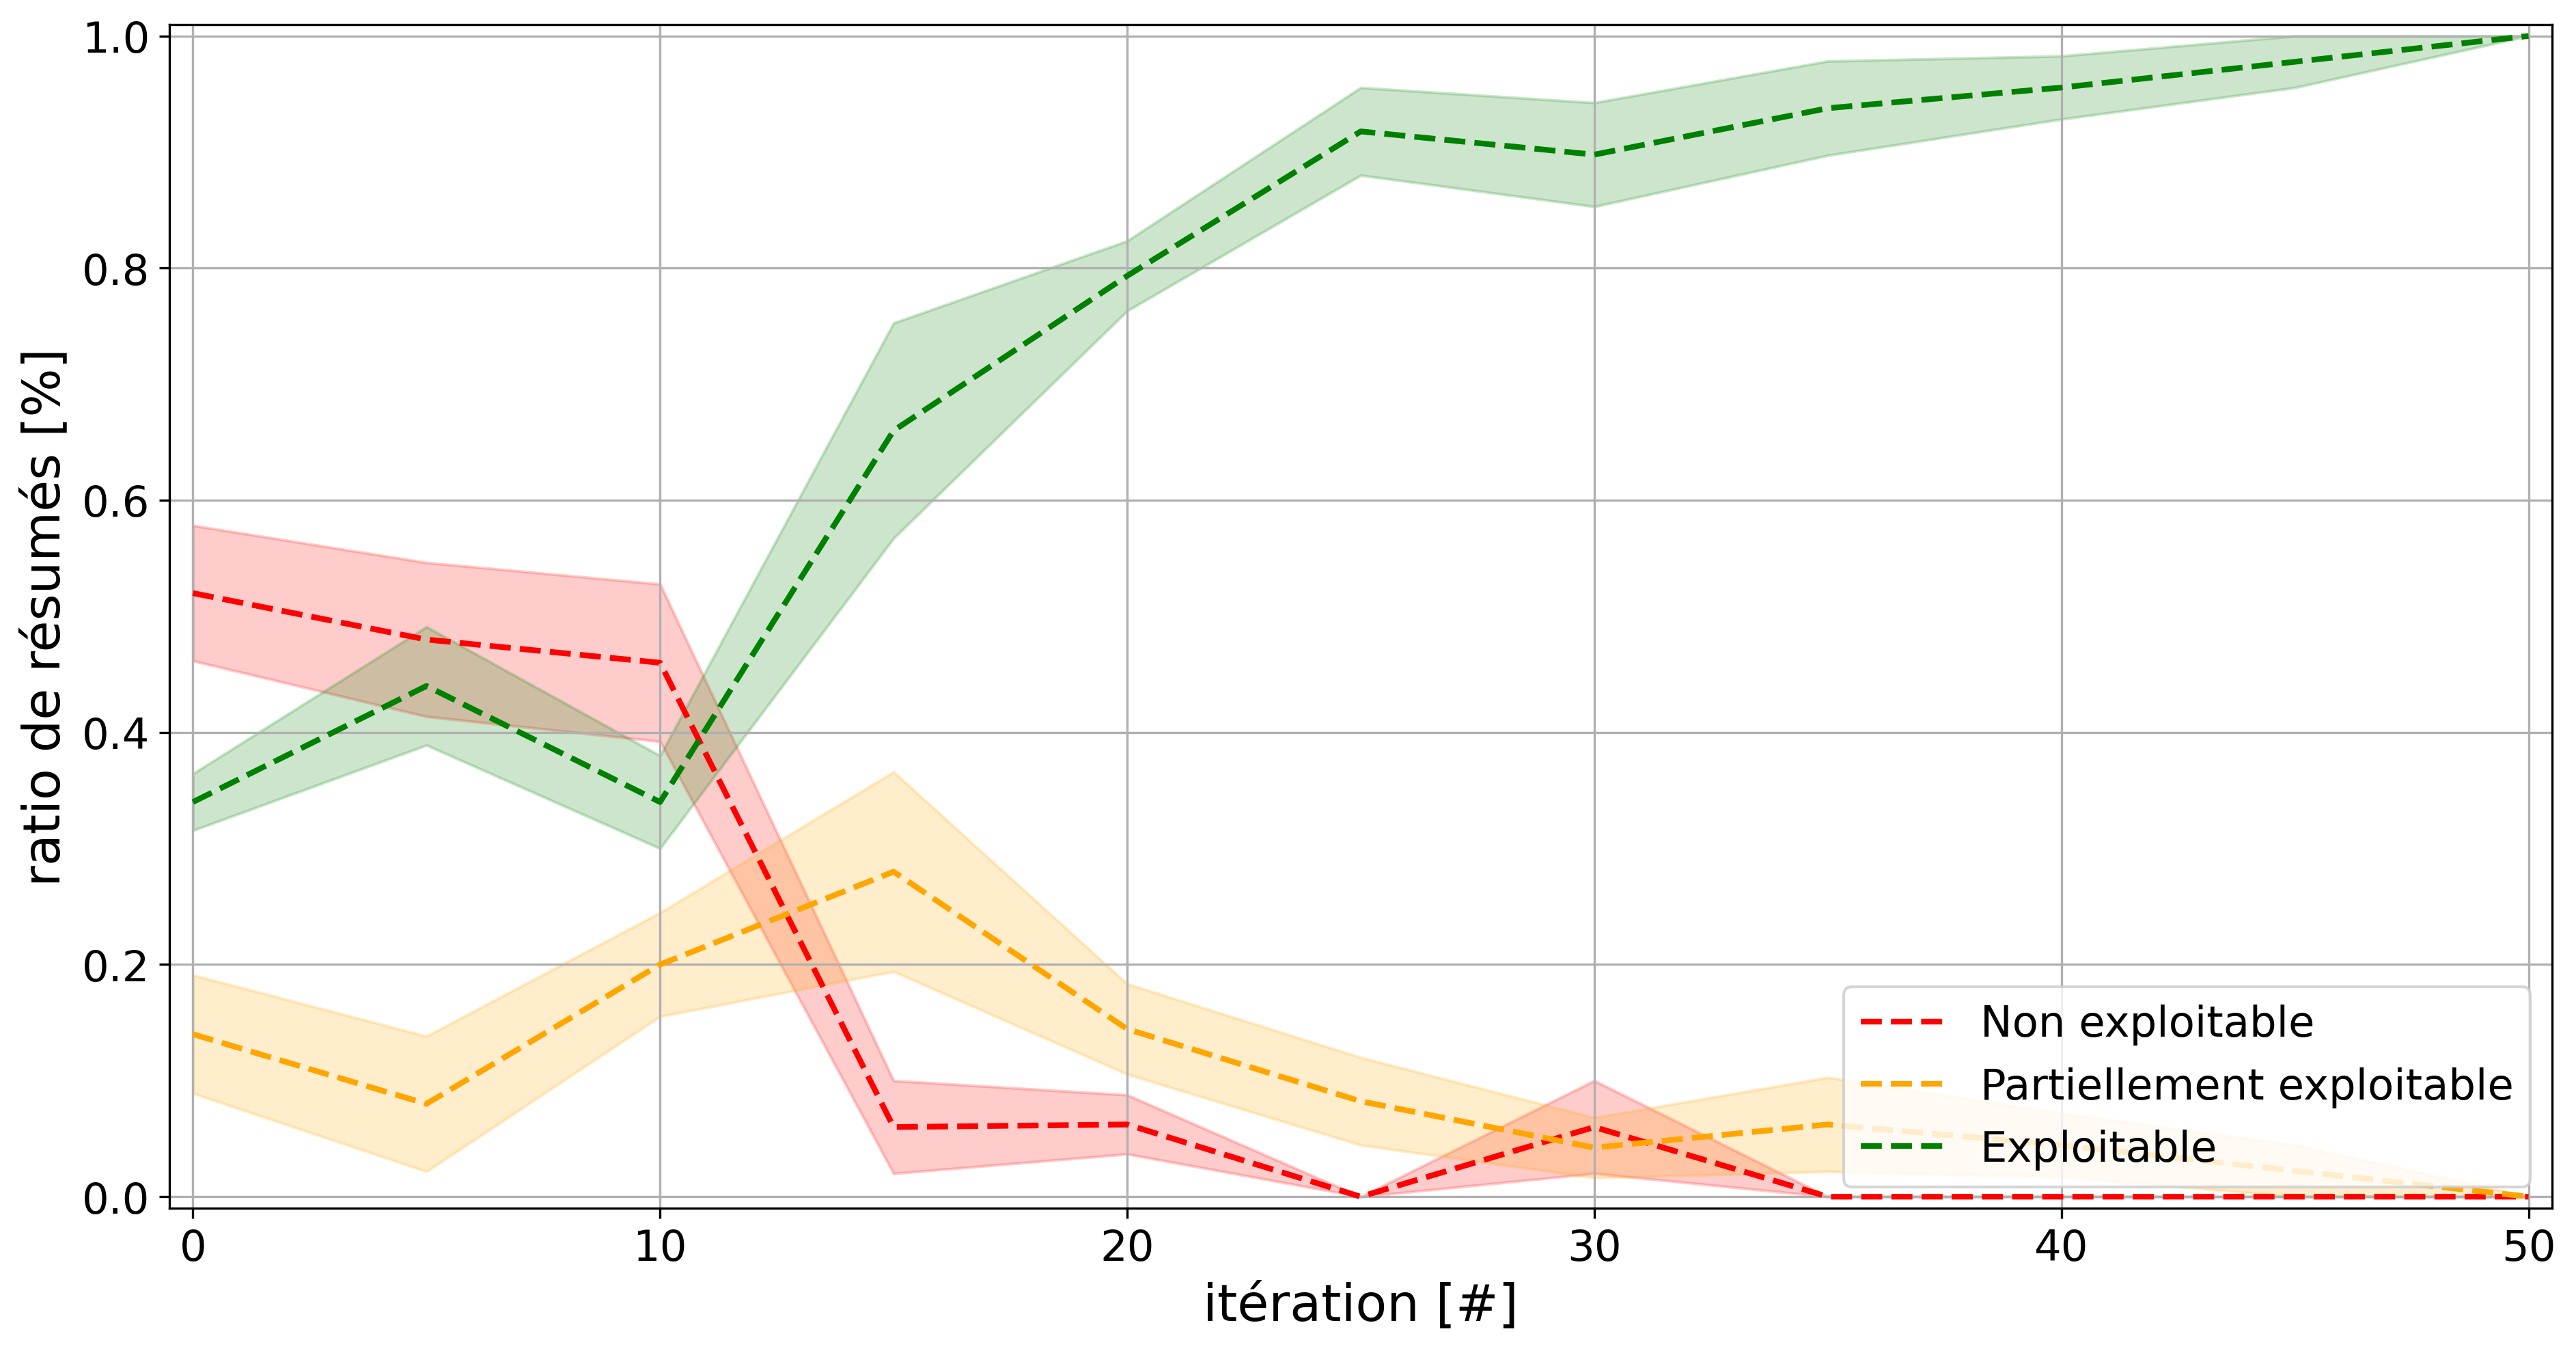
\includegraphics[width=0.95\textwidth]{figures/etude-pertinence-llm-check-resume-annotation-favori}
				\caption{Évolution de la pertinence métier moyenne en fonction du nombre d'itérations de la méthode.
				Cette pertinence, exprimée en proportion du nombre de \textit{clusters}, est estimée sur la base du résumé automatique des \textit{clusters} par un modèle de langue et est retranscrite en trois niveaux : \texttt{exploitable} en vert, \texttt{partiellement exploitable} en orange, et \texttt{non exploitable} en rouge.}
				\label{figure:4.4.3-ETUDE-PERTINENCE-RESUME-AUTOMATIQUE}
			\end{figure}

		%%% Discussion
		\subsubsection{Discussion}
			\todo[inline]{A REDIGER}
		
			% Remaques expérience utilisateur.
			\todo[inline]{A REDIGER: C'est super pratique, super accessible}
			\todo[inline]{A REDIGER: C'est parfois un peu ambigu...}
			
			% Conclusions et suggestion.
	
	
	%%%
	%%% Subsection 4.4.4: Étude de la cohérence statistique de la base d'apprentissage en cours de construction
	%%%
	%\subsection{Étude de la cohérence statistique de la base d'apprentissage en cours de construction}
	%\label{section:4.4.4-ETUDE-PERTINENCE-COHERENCE}
	%	
	%	% Objectif de l'expérience.
	%	\todo[inline]{A REDIGER: objectif de l'expérience}
	%
	%	%%% Protocole expérimental.
	%	\subsubsection{Protocole expérimental}
	%		\todo[inline]{A REDIGER}
	%		% Axiome.
	%		% Pseudo-code.
	%		% Détails de l'expérience.
	%		% Référence scripts.
	%
	%	%%% Résultats
	%	\subsubsection{Résultats obtenus}
	%		\todo[inline]{A REDIGER}
	%	
	%		% Description statistiques.
	%		
	%		% Exemple.
	%		
	%		% Figure.
	%		%
	%		\begin{figure}[!htb]
	%			\centering
	%			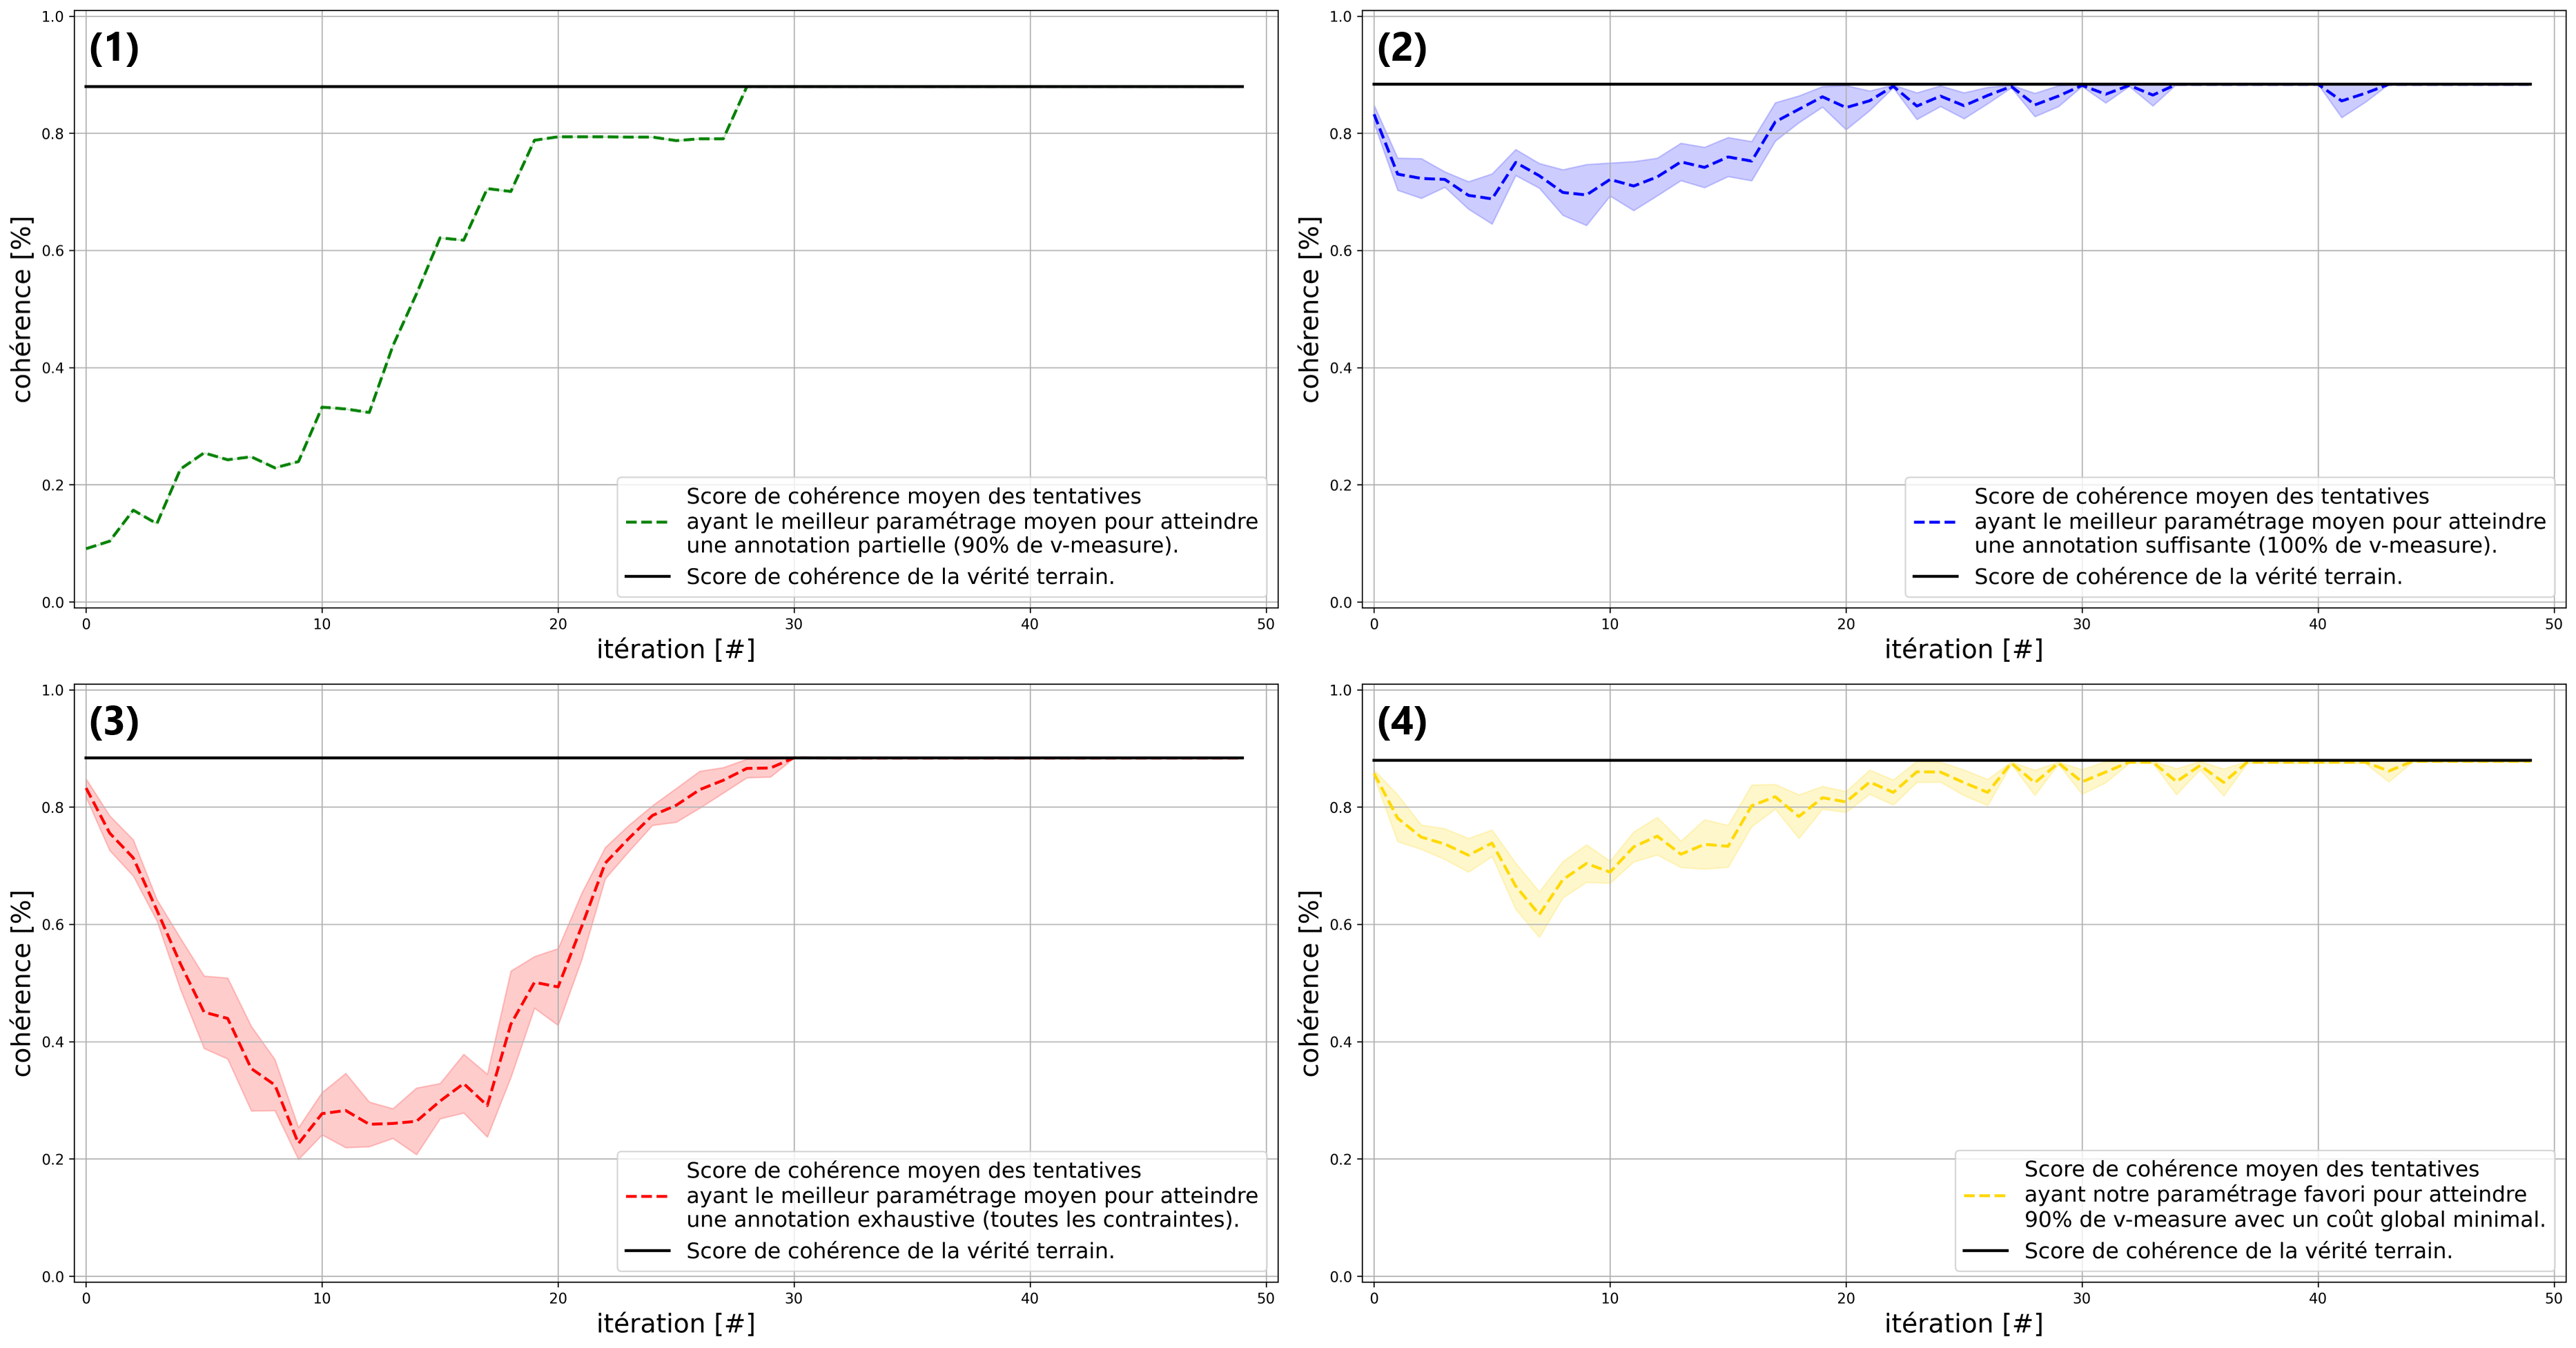
\includegraphics[width=0.95\textwidth]{figures/etude-pertinence-consistence}
	%			\caption{Évolution du score de cohérence moyen des tentatives en fonction de leur paramétrage : \textbf{(1)} meilleur paramétrage moyen une annotation partielle (\texttt{90}\% de \texttt{v-measure}), \textbf{(2)} meilleur paramétrage moyen une annotation suffisante (\texttt{100}\% de \texttt{v-measure}), \textbf{(3)} meilleur paramétrage moyen une annotation exhaustive (annoter toutes les contraintes possibles), et \textbf{(4)} paramétrage favori (\texttt{90}\% de \texttt{v-measure} avec un coût minimal). \\
	%			Note : \textit{Le score de cohérence de la vérité terrain peut varier en fonction des méthodes de prétraitements et de vectorisation utilisées.}}
	%			\label{figure:4.4.4-ETUDE-PERTINENCE-COHERENCE-ANNOTATION}
	%		\end{figure}
	%
	%	%%% Discussion
	%	\subsubsection{Discussion}
	%		\todo[inline]{A REDIGER}
	%	
	%		% Remaques expérience utilisateur.
	%		
	%		% Conclusions et suggestion.